\chapter{Results}
 
\section{Specimen Selection \& Characterization}

\subsection{Model Evaluation and Validation}

\begin{figure}[h]
\centering
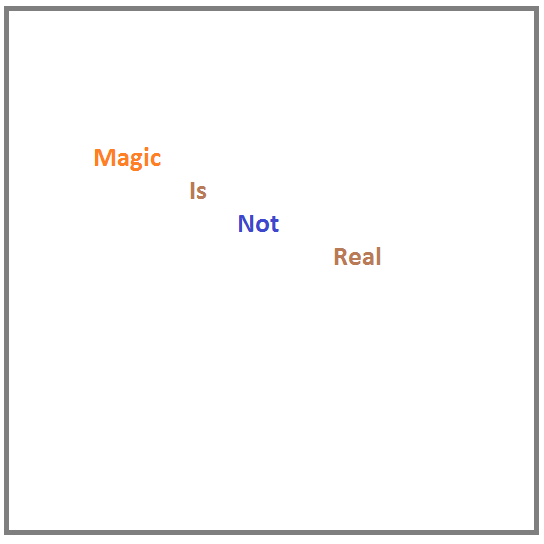
\includegraphics[width=0.5\textwidth]{figs/magic}
\caption{High score by the Game Bot.}
\end{figure}

Figure 9 is a screenshot when the car reach the finishing line and it got a score of 10269. The network was trained over 10,000 time steps and the behavior has been learned gradually. Compared to random bot, it has shown obvious better performance. For better or human level behavior, more training time steps are needed.

%%%%%%%%%%%%%%%%%%%%%%%%%%%%%%%%%%%%%%%%%%%%%%%%%%%%%%%%%%%%%%%%%%%%%%%%%%%%%%%%%%%%%%%%%%%%%%%%%%%%
\subsection{Justification}

\begin{figure}[h]
\centering
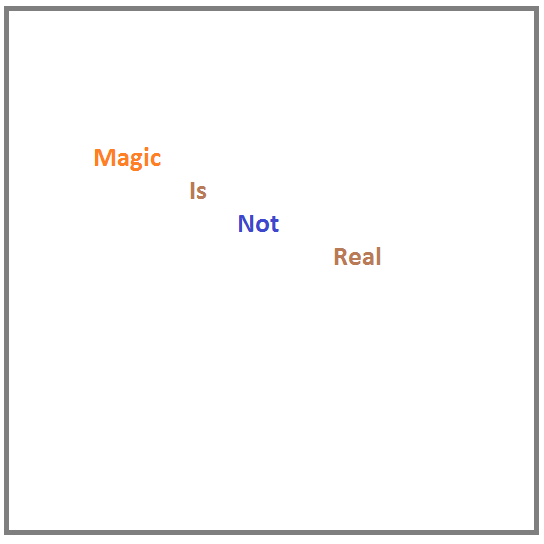
\includegraphics[width=0.5\textwidth]{figs/magic}
\caption{A comparison between DQN trained Game Bot and a random Game Bot.}
\end{figure}

The reward histories shown in Figure 10 indicates how it performs better than a random Game Bot when the DQN one is trained 100000 time steps. It proves a much better ability to earn scores or rewards though there is still a big room to improve. The Game Bot can earn as high as 10269 scores though it still usually ranks the last.


%\bibliographystyle{plainnat}
%\markright{\textit{Bibliography}}
%\renewcommand{\chaptername}{}
%\bibliography{my_references}


\vfill
